\section{Introduction}\label{sec:intro}
%% I added some background. If you consider it too technical, we can certainly remove it.
Modern machine learning and statistics deal with the problem of \emph{learning from data}: given a training dataset $\{(y_i,\xx_i)\}_{1\leq i \leq n}$ where $\xx_i \in \mathbb{R}^{d}$ is the input and $y_i \in \mathbb{R}$ is the output\footnote{When the label $y$ is given, this problem is often known as \emph{supervised learning}. We mainly focus on this paradigm throughout this paper and remark sparingly on its counterpart, \emph{unsupervised learning}, where $y$ is not given.}, one seeks a function $f: \mathbb{R}^{d} \mapsto \mathbb{R}$ from a certain function class $\mathcal{F}$ that has good prediction performance on test data. This problem is of fundamental significance and finds applications in numerous scenarios. For instance, in image recognition, the input $\xx$ (reps.~the output $y$) corresponds to the raw image (reps.~its category) and the goal is to find a mapping $f(\cdot)$ that can classify future images accurately. Decades of research efforts in statistical machine learning have been devoted to developing methods to find $f(\cdot)$ efficiently with provable guarantees. Prominent examples include linear classifiers (e.g., linear$\,$/$\,$logistic regression, linear discriminant analysis), kernel methods (e.g., support vector machines), tree-based methods (e.g., decision trees, random forests), nonparametric regression (e.g., nearest neighbors, local kernel smoothing), etc. Roughly speaking, each aforementioned method corresponds to a different function class $\mathcal{F}$ from which the final classifier $f(\cdot)$ is chosen.

Deep learning~\citep{lecun2015deep}, in its simplest form, proposes the following \emph{compositional} function class:
\begin{equation}\label{model:1}
\left\{f(\xx; \btheta) = \bW_{L} \bsigma_L(\bW_{L-1}\cdots \bsigma_{2}(\bW_2 \bsigma_1(\bW_1 \xx))) \;\big| \;\btheta = \{\bW_1,\ldots, \bW_{L}\}\right\}.
\end{equation}
Here, for each $1\leq l \leq L$, $\bsigma_\ell(\cdot)$ is some nonlinear function, and $\btheta = \{\bW_1,\ldots, \bW_{L}\}$ consists of matrices with appropriate sizes. Though simple, deep learning has made significant progress towards addressing the problem of learning from data over the past decade. Specifically, it has performed close to or better than humans in various important tasks in artificial intelligence, including image recognition~\citep{he2016deep}, game playing~\citep{silver2017mastering}, and machine translation~\citep{wu2016google}. Owing to its great promise, the impact of deep learning is also growing rapidly in areas beyond artificial intelligence; examples include statistics~\citep{bauer2017deep, schmidt2017nonparametric, liang2017well, romano2018deep,gao2018robust}, applied mathematics~\citep{weinan2017deep, chen2018neural}, clinical research~\citep{de2018clinically}, etc.

%The widespread use of deep leaning has lead to a myriad of frameworks (e.g.~Tensroflow~\citep{tensorflow2015-whitepaper}, PyTorch~\citep{paszke2017automatic}) for researchers and practitioner to build and deploy the models efficiently.

%Within the realm of artificial intelligence, deep learning has performed close to or better than humans in image recognition. In games such as Go and Chess, methods trained with deep learning are much better than humans, even without any input of human knowledge. In machine translation, deep learning has made great improvement over existing methods. Apart from the field of artificial intelligence, deep learning has shown huge promises.

% from a certain function class $\mathcal{F}$


%Deep learning has been recognized as one of the most important methods in artificial intelligence, and its impact is growing in statistics~\citep{bauer2017deep, schmidt2017nonparametric, liang2017well, romano2018deep}, applied mathematics~\citep{weinan2017deep, chen2018neural}, statistical physics, clinical research~\citep{de2018clinically}, etc. Within the realm of artificial intelligence, deep learning has drawn huge research interest and achieved significant progress in various important tasks since 2012,. In image recognition, deep learning has performed close to or better than humans. In games such as Go and Chess, methods trained with deep learning are much better than humans, even without any human knowledge input. In machine translation, deep learning has made great improvement over existing methods. Apart from the field of artificial intelligence, deep learning has shown huge promises.
\begin{table}[htb]
\caption{Winning models for ILSVRC image classification challenge.}
\label{tab:intro}
\begin{center}
\begin{tabular}{|c|c|c|c|c|}
\hline
Model & Year & \# Layers & \# Params & Top-5 error \\
%\hhline{|=|=|=|=|=|}
\hline
Shallow & $<2012$ & --- & --- & $>25\%$ \\
\hline
AlexNet & $2012$ & $8$ & $61$M & $16.4\%$ \\
\hline
VGG19 & $2014$ & $19$ & $144$M & $7.3\%$ \\
\hline
GoogleNet & $2014$ & $22$ & $7$M & $6.7\%$ \\
\hline
ResNet-$152$ & $2015$ & $152$ & $60$M & $3.6\%$ \\
\hline
\end{tabular}
\end{center}
\end{table}
To get a better idea of the success of deep learning, let us take the ImageNet Challenge~\citep{ILSVRC15} (also known as ILSVRC) as an example. In the classification task, one is given a training dataset consisting of 1.2 million color images with $1000$ categories, and the goal is to classify images based on the input pixels. The performance of a classifier is then evaluated on a test dataset of 100 thousand images, and in the end the top-5 error\footnote{The algorithm makes an error if the true label is not contained in the $5$ predictions made by the algorithm.} is reported. Table~\ref{tab:intro} highlights a few popular models and their corresponding performance. As can be seen, deep learning models (the second to the last rows) have a clear edge over shallow models (the first row) that fit linear models$\,$/$\,$tree-based models on handcrafted features. This significant improvement raises a foundational question:

\begin{itemize}
\centering
\item[] \mbox{\emph{Why is deep learning better than classical methods on tasks like image recognition?}}
\end{itemize}



%\begin{center}
%\emph{why is deep learning better than classical methods on tasks like image recognition?}
%\end{center}

%For comparison, a Stanford Ph.D. student achieved a $5.1\%$ error on the same task.

%Clearly, generally over-parametrized and deep models have superior performance compared with shallow models\footnote{Shallow models are typically feature extraction followed by linear/nonlinear SVMs, which are used in ILSVRC classification challenge before 2012.}.


%One well-known example of the success of deep learning is the ImageNet Challenge~\citep{ILSVRC15}, where the goal is to classify images based on input pixels.  In the classification task, the training dataset consists of 1.2 million color images (typically, $256 \times 256$) with $1000$ categories. The performance of a classifier is evaluated on a test dataset of 100 thousands images, and the top-5 error\footnote{The top-5 error refers to the ratio of mismatch between the true label $y$ and $5$ labels predicted by an algorithm (a mismatch is counted if $y$ is not any of the $5$ predicted labels). It is a more tolerant criterion than the usual classification/top-1 error.} is reported. In Table~\ref{tab:intro}, we highlight several famous models and their performance, among which the last two models will be discussed in Section~\ref{sec:skip}. Clearly, generally over-parametrized and deep models have superior performance compared with shallow models\footnote{Shallow models are typically feature extraction followed by linear/nonlinear SVMs, which are used in ILSVRC classification challenge before 2012.}.





%\subsection{Classical methods revisited}
%
%Before delving into deep learning, let us imagine what a data analyst would do to attack a classification problem in the traditional way. The data analyst may start with simple visualization and logistic regression (or support vector machine). After realizing the nonlinear nature of the data, he$\,$/$\,$she carefully reexamines the task and falls into thoughts, before coming up with key structural assumptions. For example, the density function is supposed to be quite smooth, or there should be a sparse representation of the data after proper transformation, and so on. With these assumptions in mind, the data analyst then diligently spends hours working on feature construction, before finally running standard packages from \texttt{R}, \texttt{MATLAB}, or \texttt{Python} to fit a model.
%
%%One of the most popular methods for classification (resp.~regression) is logistic regression (resp.~linear regression). Due to its linear nature, it can be very restrictive in modeling nonlinear decision boundaries in complex problems such as image classification. Decades of research efforts in nonparametric statistics, semiparametric statistics, machine learning, etc., have been devoted to discovering routes in the world of nonlinearity. Prominent examples include basis expansion (e.g., splines, wavelets, reproducing kernel Hilbert spaces)~\citep{wahba1990spline, daubechies1992ten}, local kernel smoothing (e.g., nearest neighbors, local regression, polynomial smoothing)~\citep{fan2018local, loader2006local}, tree-based methods (e.g., decision trees, random forests)~\citep{breiman1984classification, breiman2001random}, etc.
%
%%{\scriptsize
%%\begin{equation*}
%%\begin{array}{lc}
%%\text{Known structure} & \left\{ \begin{array}{lcl} \text{smoothness} & \longrightarrow & \text{kernel smoothing, fourier/wavelets transformation} \\ \text{sparsity} & \longrightarrow & \text{thresholding}, \ell_1 \text{-, SCAD-regularization, basis pursuit} \\ \text{low rank} & \longrightarrow & \text{PCA, SDP, nuclear-norm minimization} \\ \cdots & \longrightarrow & \cdots \end{array} \right. \\
%%\text{Unclear structure?} & \begin{array}{lcl} & \hspace{-43mm}  \longrightarrow & \text{deep learning}  \end{array}
%%\end{array}
%%\end{equation*}
%%}
%
%Indeed, if a problem has a certain known structure, such as smoothness, sparsity, and low-rankness, then one can usually devise near-optimal statistical methods in the minimax sense~\citep{stone1982optimal, donoho1994ideal, candes2009power,chen2019noisy}. However, for datasets such as images and natural languages, it is not \emph{a priori} obvious what structure best characterizes these datasets. In addition, classical methods do not seem to be flexible enough to model the nonlinear dependency between $y$ and $\xx$ for these datasets.
%
%The success of deep learning is an indication that deep learning models represent a very different class of functions that are suitable for highly complex datasets. In particular, while the \textit{curse of dimensionality} is often encountered with the class of smooth functions, deep learning excels at handling many high-dimensional data (images, videos, etc.). In general, the curse of dimensionality refers to the phenomenon that the sample and computational complexities have to grow exponentially with the dimension $d$ to achieve a given accuracy. For example, in nonparametric regression, the optimal convergence rate for a Lipschitz regression function is $O(n^{-2/(2+d)})$. Therefore to obtain a small error $\varepsilon$, the number of samples has an exponential dependence on $d$~\citep{stone1982optimal}. Smoother functions, e.g., functions with all derivatives up to the $m$-th order, can have a better convergence rate $O(n^{-2m/(2m+d)})$; however, it is often unrealistic to expect high smoothness in high-dimensional real data. Apart from the sample complexity, many optimization problems require computational cost that is exponential in terms of the input dimension in the worst case (a.k.a.~NP-hardness)~\citep{arora2009computational}. Nevertheless, generic algorithms (e.g., stochastic gradient descent, \citealp{robbins1951stochastic}) are powerful enough to find a good classifier with the deep learning models despite its large size. Due to the huge difference, deep learning can be regarded as a new framework for statistical modeling and methods.
%
%%These pessimistic results on exponential dependency are related to a very simple intuition: generally it requires $O((1/\varepsilon)^d)$ evaluations on a grid of a cube to determine a function within $\varepsilon$ tolerance \citep{donoho2000high}.
%
%%Deep learning is not only good at representing complex functions, but also efficient in finding them. This is perhaps more surprising, since the complexities of deep learning models are much higher than classical methods.
%
%%In particular, the \textit{curse of dimensionality} is one difficulty often encountered under the classical structural assumptions. In general, it refers to the phenomenon that sample and computational complexities have to grow exponentially with the dimension $d$ to achieve a given accuracy. For example, in nonparametric regression, the optimal convergence rate for a Lipschitz regression function is $O(n^{-2/(2+d)})$. Therefore to obtain a small error $\varepsilon$, the number of samples has an exponential dependence on $d$~\citep{stone1982optimal}. Smoother functions, e.g., functions with all derivatives up to the $m$-th order, can have better convergence rate $O(n^{-2m/(2m+d)})$, however, it is often unrealistic to expect high smoothness in high-dimensional real data.  Apart from the sample complexity, in the worst case, many optimization problems require computational cost that is exponential in terms of the input dimension (a.k.a.~NP-hardness)~\citep{arora2009computational}. These pessimistic results on exponential dependency are related to a very simple intuition: generally it requires $O((1/\varepsilon)^d)$ evaluations on a grid of a cube to determine a function within $\varepsilon$ tolerance \citep{donoho2000high}.
%
%%The success of deep learning is an indication that deep learning models represent a very different class of functions that are suitable for highly complex datasets. Moreover, on the computational side, generic algorithms (e.g., stochastic gradient descent~\citep{robbins1951stochastic}) are powerful enough to find a good classifier, despite the large size of the model. Due to the huge difference, deep learning can be regarded as a new framework for statistical modeling and methods.
%%
%%%In a way, deep learning sheds new lights to the \textit{curse of dimensionality} by learning certain complicated nonlinearity efficiently.
%%
%%%Deep learning models do not seem to suffer from this curse of dimensionality, likely because they represent a different class of functions that are suitable for many real datasets.
\begin{figure}
\centering
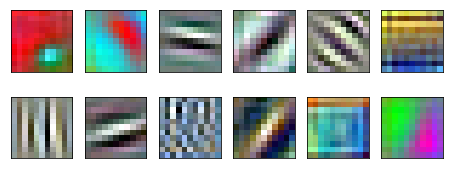
\includegraphics[width = 0.75\textwidth]{ImagnetFilterVisualization2by6}
\caption{Visualization of trained filters in the first layer of AlexNet. The model is pre-trained on ImageNet and is downloadable via PyTorch package \texttt{torchvision.models}. Each filter contains $11 \times 11 \times 3$ parameters and is shown as an RGB color map of size $11 \times 11$.}\label{fig:vis}
\end{figure}
\subsection{Intriguing new characteristics of deep learning}

It is widely acknowledged that two indispensable factors contribute to the success of deep learning, namely (1) huge datasets that often contain millions of samples and (2) immense computing power resulting from clusters of graphics processing units (GPUs). Admittedly, these resources are only recently available: the latter allows to train larger neural networks which reduces biases and the former enables variance reduction. However, these two alone are not sufficient to explain the mystery of deep learning due to some of its ``dreadful'' characteristics: (1) \emph{over-parametrization}: the number of parameters in state-of-the-art deep learning models is often much larger than the sample size (see Table~\ref{tab:intro}), which gives them the potential to overfit the training data, and (2) \emph{nonconvexity}: even with the help of GPUs, training deep learning models is still NP-hard~\citep{arora2009computational} in the worst case due to the highly {nonconvex} loss function to minimize. In reality, these characteristics are far from nightmares. This sharp difference motivates us to take a closer look at the salient features of deep learning, which we single out a few below. %\cm{We should shorten the introduction and the bullet points.}


%\begin{figure}
%\centering
%\begin{tabular}{cc}
%\includegraphics[width = 0.3\textwidth]{Figure/MNIST_whole.pdf} & \includegraphics[width = 0.3\textwidth]{Figure/my_visualization}  \tabularnewline
%(a) One-to-many & (b) Many-to-one
%\end{tabular}
%\caption{Vanilla RNNs with different inputs/outputs settings. (a) has one input but multiple outputs; (b) has multiple inputs but one output; (c) has multiple inputs and outputs. Note that the parameters are shared across time steps.}\label{fig:mnist}
%\end{figure}

%The departure from conventional wisdoms and classical methods generates many intriguing new phenomena.
%All of this motivates us to take a closer look at what is new in deep learning and what are the connections with conventional methods and wisdoms. Below we single out three salient features of deep learning.

\subsubsection{Depth}
Deep learning expresses complicated nonlinearity through composing many nonlinear functions; see~(\ref{model:1}). The rationale for this multilayer structure is that, in many real-world datasets such as images, there are different levels of features and lower-level features are building blocks of higher-level ones. See~\cite{yosinski2015understanding} for a visualization of trained features of convolutional neural nets; here in Figure~\ref{fig:vis}, we sample and visualize weights from a pre-trained AlexNet model. This intuition is also supported by empirical results from physiology and neuroscience~\citep{hubel1962receptive, abbasi2018deeptune}. The use of function composition marks a sharp difference from traditional statistical methods such as projection pursuit models \citep{friedman1981projection} and multi-index models \citep{li1991sliced, cook2007fisher}. It is often observed that depth helps efficiently extract features that are representative of a dataset. In comparison, increasing width (e.g., number of basis functions) in a shallow model leads to less improvement. This suggests that deep learning models excel at representing a very different function space that is suitable for complex datasets.


%Although each nonlinear component a simple element-wise nonlinear function, stacking many such functions allows to model complicated nonlinearity well.

%traditional methods often require hand-crafted features that are not flexible enough for a task.
%This suggests that deep learning models have great representation power
%where much focus is on structured smoothness (e.g., Sobolev space) and structure sparsity (e.g., sparse signals, low rank).
%This may explain why the curse of dimensionality, usually found in statistics, is not observed in deep learning.
%Deep models bring not only representational power, but new computational challenges as well.
%New challenges arise for deep models, and they are particularly acute in the computational aspect. For example, as the number of composed functions increases, training can be very slow; also the gradients are usually vanishing or exploding, which leads to numerical instability~\citep{hochreiter1991untersuchungen, hochreiter2001gradient}. Many techniques are proposed to address these issues: for example, weight sharing and downsampling speed up the computation, and batch normalization and skip connections stabilize gradient flows (Section~\ref{sec:pop} and~\ref{sec:opt}).
%two perspectives, namely its representation power and generalization power. The former refers to the capacity of deep neural nets to approximate functions (i.e., what is the function space) and the latter refers to the effectiveness of controlling out-of-sample errors (i.e., why they achieve small test errors).

%Moreover, deep learning algorithms can find good representations and thus good prediction results with reasonable computational costs. We identify three important characteristics of deep learning in the following. The first two will be highlighted in this paper.

%\subsubsection{Over-parametrization.}

\subsubsection{Algorithmic regularization}
%\subsubsection{Entanglement with training algorithms}
The statistical performance of neural networks (e.g., test accuracy) depends heavily on the particular optimization algorithms used for training~\citep{NIPS2017_7003}. This is very different from many classical statistical problems, where the related optimization problems are less complicated. For instance, when the associated optimization problem has a relatively simple structure (e.g., convex objective functions, linear constraints), the solution to the optimization problem can often be unambiguously computed and analyzed. However, in deep neural networks, due to over-parametrization, there are usually many local minima with different statistical performance \citep{li2018visualizing}. Nevertheless, common practice runs stochastic gradient descent with random initialization and finds model parameters with very good prediction accuracy. %For example, the choice of batch size has significant influence on test accuracy (see Section~\ref{sec:opt}). This phenomenon calls for understanding optimization algorithms from the statistical lens.\\


%Recent research suggests that certain optimization algorithms, such as gradient descent and stochastic gradient descent, works well with over-parametrized models---with stochastic gradient descent, a huge model does not lead to inferior generalization power (test error). Also, the algorithms exhibit \textit{implicit regularization}, which means that even without explicit regularization such at $\ell_2$ regularizers or $\ell_1$ regularizers, optimization algorithms can produce regularized functions/classifiers $f_{\btheta}$.

\subsubsection{Implicit prior learning}
It is well observed that deep neural networks trained with only the raw inputs (e.g., pixels of images) can provide a useful representation of the data. This means that after training, the units of deep neural networks can represent features such as edges, corners, wheels, eyes, etc.; see~\cite{yosinski2015understanding}. Importantly, the training process is automatic in the sense that no human knowledge is involved (other than hyper-parameter tuning). This is very different from traditional methods, where algorithms are designed after structural assumptions are posited. %Because of this reason, tasks involving complex large-scale datasets can become more efficient in terms of labor investment.
It is likely that training an over-parametrized model efficiently learns and incorporates the prior distribution $p(\xx)$ of the input, even though deep learning models are themselves discriminative models. With automatic representation of the prior distribution, deep learning typically performs well on similar datasets (but not very different ones) via transfer learning.

%\subsubsection{Over parametrization and implicit prior.}

%Over parametrization can drive easily the training errors to zero. This is traditionally regarded as over-fitting and can have an adverse effect on the generalization error (prediction erro).  However, in highly complex high-dimensional model, the biases are the key factors in prediction error and are hard to control. Overparameterized models are typically have lower biases than, for example, the nearest neighborhood learning. Since the algorithms are trained based on a large amount of samples, this incorporates implicitly the prior of the data, so long as the training examples are not biasedly sampled, namely the testing samples (features) are similar to the those from the training samples.  When this over-parametrization is coupled with the aforementioned implicit regularization, the variance does not increase as much.  Indeed, the generalization error controlled by two factors: training errors and Rademacher complexity of the model {\bf Ref?}.  For overparametrized models, the first term is nearly zero. Yet, overparametrized models do not need many steps of iterations of gradient steps to drive the training error to zero and hence its Rademacher complexity is also controlled.  This provides a heuristic explanation the complex story behind deep learning's successes.


%new models and algorithms that enable scalable training of deep neural nets. While the first two factors involve resources that are only recently available, the third requires clever algorithmic insights---in this aspect, research communities have recently contributed many novel ideas, including residual nets, dropout training, generative models, batch normalization, etc. %Nevertheless, the architectures of deep learning, such as the deep neural networks and recurrent neural networks, are not completely new ideas.
%These innovations are built upon ideas and methods developed over several decades. Deep learning architectures and training can be traced back to as early as the perceptron algorithm~\citep{rosenblatt1958perceptron}, and they gradually evolved into the modern appearance~\citep{fukushima1979neural, lecun1989backpropagation, krizhevsky2012imagenet}. For a comprehensive monograph and the history, we refer the readers to~\citep{lecun2015deep, schmidhuber2015deep, deeplearningbook}.
%%The architectures of deep learning, such as the deep neural networks and recurrent neural networks, are not completely new ideas. They can be traced back to as early as the perceptron algorithm~\citep{rosenblatt1958perceptron}, and gradually evolved into its modern appearance~\citep{fukushima1979neural, lecun1989backpropagation, krizhevsky2012imagenet}. However, there are important resources that are only recently available and are critical to the success of deep learning: (1) huge datasets that often contain millions of samples, (2) immense computing power, especially from graphics processing units (GPUs). Besides, research communities have contributed many novel ideas, including, notably, dropout training, residual nets, generative adversarial nets, batch normalization, etc. For a comprehensive monograph or the history, we refer the readers to~\citep{lecun2015deep, schmidhuber2015deep}.
%
%Fundamentally, deep learning is a method for the classical statistical problem: given a training data $\{(\xx_i,y_i)\}_{1\leq i \leq n}$ where $\xx_i \in \mathbb{R}^{d}$ is the (raw) input and $y_i \in \mathbb{R}$ (categorical or real-valued) is the output, we want to find a function $f_{\btheta}: \mathbb{R}^{d} \mapsto \mathbb{R}$ with good prediction performance on unseen data. As with standard approaches in statistics and machine learning, the parameters $\btheta$ are determined by minimizing certain loss functions. Often, the input dimension $d$ is very large (e.g., the number of pixels in a color image), and the dependence between $y_i$ and $\xx_i$ is highly nonlinear (e.g., predicting image categories based on raw pixels); these together pose great challenges for traditional approaches. Deep learning uses a very large model with many layers, and the total number of parameters as large as hundreds of millions. A vanilla feed-forward neural network has the following structure:
%\begin{equation}\label{model:1}
%f_{\btheta}(\xx) = \bA_\ell \bsigma_*(\cdots \bsigma_*(\bA_2 \bsigma_*(\bA_1 \xx))),
%\end{equation}
%where $\bA_1,\cdots, \bA_\ell$ are matrices with appropriate sizes and $\bsigma_*(\cdot)$ is a nonlinear function applied in an element-wise fashion.
%
%With reasonably good computing resources, deep learning usually achieves a small training error (in-sample error) on the training data, and perhaps surprisingly, a small test error (out-of-sample error) on separate test data. This clearly stands in contrast with the traditional wisdom, which typically works with smaller models to avoid overfitting. Before suggesting perspectives to explain this apparent discrepancy, we first have a look at classical statistical methods.
%
%\subsubsection{Classical methods for nonlinearity.}
%
%One of the most popular methods for classification (resp.~regression) is logistic regression (resp.~linear regression). Due to its linear nature, it can be very restrictive in modeling nonlinear decision boundaries in complex problems such as image classification. Decades of research efforts in nonparametric statistics, semiparametric statistics, machine learning, etc., have been devoted to discovering routes in the world of nonlinearity. Prominent examples include basis expansion (e.g., splines, wavelets, reproducing kernel Hilbert spaces)~\citep{wahba1990spline, daubechies1992ten}, local kernel smoothing (e.g., nearest neighbors, local regression, polynomial smoothing)~\citep{fan2018local, loader2006local}, tree-based methods (e.g., decision trees, random forests)~\citep{breiman1984classification, breiman2001random}, etc.
%
%\begin{equation*}
%\begin{array}{lc}
%\text{Known structure} & \left\{ \begin{array}{lcl} \text{smoothness} & \longrightarrow & \text{kernel smoothing, fourier/wavelets transform} \\ \text{sparsity} & \longrightarrow & \text{thresholding}, \ell_1 \text{-regularization, basis pursuit} \\ \text{low rank} & \longrightarrow & \text{PCA, SDP, nuclear-norm minimization} \\ \cdots & \longrightarrow & \cdots \end{array} \right. \\
%\text{Unclear structure?} & \begin{array}{lcl} & \hspace{-31mm}  \longrightarrow & \text{deep learning}  \end{array}
%\end{array}
%\end{equation*}
%
%If a problem has a certain known structure, such as smoothness, sparsity, and low rank, then one can usually devise (near-)optimal statistical methods in the minimax sense~\citep{stone1982optimal, donoho1994ideal, candes2009power}. However, for datasets such as images and natural languages, it is not \emph{a priori} obvious what structure best characterizes these datasets. Even with hand-crafted features, the resulting model can be unsatisfactory. For these datasets, classical methods do not seem to be flexible enough to handle nonlinearity.
%
%In particular, the \textit{curse of dimensionality} is one difficulty often encountered under the classical structural assumptions. In general, it refers to the phenomenon that sample and computational complexities have to grow exponentially with the dimension $d$ to achieve a given accuracy. For example, in nonparametric regression, the optimal convergence rate for a Lipschitz regression function is $O(n^{-2/(2+d)})$. Therefore to obtain a small error $\varepsilon$, the number of samples has an exponential dependence on $d$~\citep{stone1982optimal}. Smoother functions, e.g., functions with all derivatives up to $m$th order, can have better convergence rate $O(n^{-2m/(2m+d)})$, however, it is often unrealistic to expect high smoothness in high-dimensional real data.  Apart from the sample complexity, in the worst case, many optimization problems require computational cost that is exponential in terms of the input dimension (a.k.a.\ NP-hardness)~\citep{arora2009computational}. These pessimistic results on exponential dependency are related to a very simple intuition: generally it requires $O((1/\varepsilon)^d)$ evaluations on a grid of a cube to determine a function within $\varepsilon$ tolerance.
%
%The success of deep learning is an indication that deep learning models represent a very different class of functions that are suitable for highly complex datasets. Moreover, on the computational side, gradient-based methods are generally powerful enough to find a good classifier, despite the large size of the model. Due to the huge difference, deep learning can be regarded as a new framework for statistical modeling and methods.
%
%%In a way, deep learning sheds new lights to the \textit{curse of dimensionality} by learning certain complicated nonlinearity efficiently.
%
%%Deep learning models do not seem to suffer from this curse of dimensionality, likely because they represent a different class of functions that are suitable for many real datasets.
%
%\subsubsection{Characteristics of deep learning.}
%
%%Despite its empirical success, theoretical justifications for this is still at infancy. Below we summarizes the efforts which have been made towards explaining the mystery of deep learning, namely its representation power and generalization power. The former refers to the capacity of deep neural nets to approximate functions, and the latter refers to the effectiveness of controlling out-of-sample errors.
%
%
%%Another interesting characteristic of deep neural nets that will not be covered in this paper is automatic feature extraction. While classical statistical methods require pre-specified features (basis, dictionaries,
%

\begin{figure}
\centering
\begin{tabular}{cc}
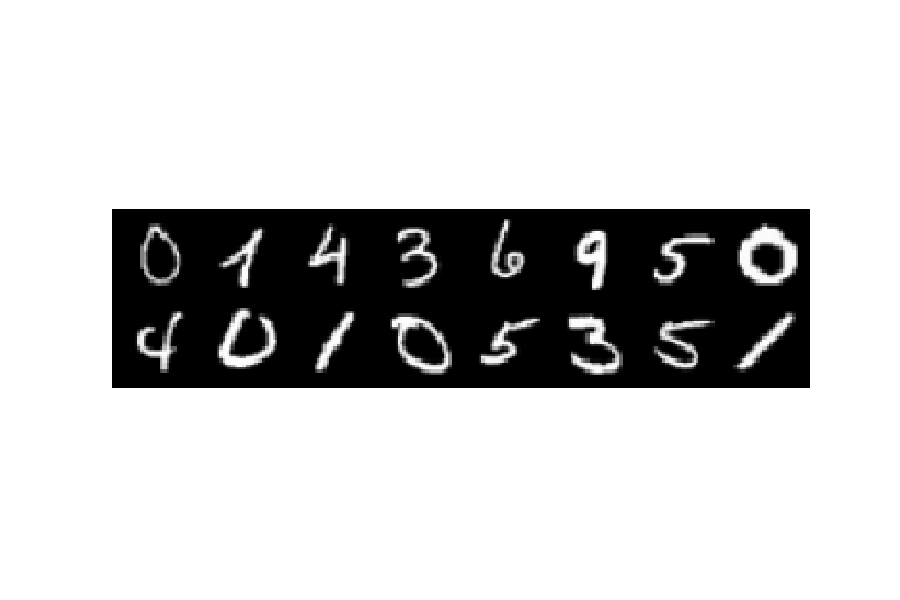
\includegraphics[width = 0.45\textwidth]{MNIST.pdf} & 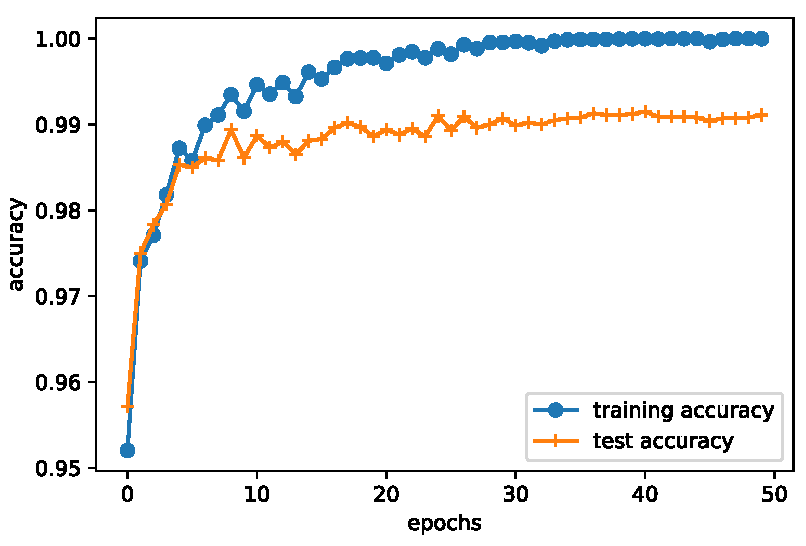
\includegraphics[width = 0.45\textwidth]{train_test_accuracy.pdf}    \tabularnewline
(a) MNIST images & (b) training and test accuracies
\end{tabular}
\caption{(a) shows the images in the public dataset MNIST; and (b) depicts the training and test accuracies along the training dynamics. Note that the training accuracy is approaching $100\%$ and the test accuracy is still high (no overfitting). }\label{fig:mnist}
\end{figure}



\subsection{Towards theory of deep learning}

Despite the empirical success, theoretical support for deep learning is still in its infancy. Setting the stage, for any classifier $f$, denote by $\mathbb{E}(f)$ the expected risk on fresh sample (a.k.a.~test error, prediction error or generalization error), and by $\mathbb{E}_n(f)$ the empirical risk$\,$/$\,$training error averaged over a training dataset. Arguably, the key theoretical question in deep learning is %\cm{The introduction here is not mathematically and a bit unclear to those who do not have previous experience with learning theory.}
\begin{center}
\emph{why is $\mathbb{E}(\hat{f}_{n})$ small, where $\hat{f}_{n}$ is the classifier returned by the training algorithm?}
\end{center}

We follow the conventional approximation-estimation decomposition (sometimes, also bias-variance tradeoff) to decompose the term $\mathbb{E}(\hat{f}_{n})$ into two parts.
Let $\cF$ be the function space expressible by a family of neural nets.
Define $f^* = \argmin_f \mathbb{E}(f)$ to be the best possible classifier and $f^*_{\cF} = \argmin_{f \in \cF} \mathbb{E}(f)$ to be the best classifier in $\cF$. Then, we can decompose the excess error $\cE \triangleq \mathbb{E}(\hat f_n) - \mathbb{E}(f^*)$ into two parts:
\begin{equation}
\cE = \underbrace{\mathbb{E}(f^*_{\cF}) - \mathbb{E}(f^*)}_{\text{approximation error}} ~ + ~ \underbrace{\mathbb{E}(\hat f_n) - \mathbb{E}(f^*_{\cF})}_{\text{estimation error}}.\label{eq:error_decomposition}
\end{equation}
Both errors can be small for deep learning (cf. Figure~\ref{fig:mnist}), which we explain below.
%where the approximation error is governed by its representation power and the estimation error is related to its generalization ability.
\begin{itemize}
\item{The \emph{approximation error} is determined by the function class $\cF$. Intuitively, the larger the class, the smaller the approximation error. Deep learning models use many layers of nonlinear functions (Figure~\ref{fig:FFNN})that can drive this error small. Indeed, in Section~\ref{sec:approx}, we provide recent theoretical progress of its representation power. For example, deep models allow efficient representation of interactions among variable while shallow models cannot.
}
\item{The \emph{estimation error} reflects the generalization power, which is influenced by both the complexity of the function class $\mathcal{F}$ and the properties of the training algorithms. Interestingly, for \emph{over-parametrized} deep neural nets, stochastic gradient descent typically results in a near-zero  training error (i.e., $\mathbb{E}_{n}(\hat{f}_{n})\approx 0$; see e.g. left panel of Figure~\ref{fig:mnist}). Moreover, its generalization error $\mathbb{E}(\hat{f}_{n})$ remains small or moderate. This ``counterintuitive'' behavior suggests that for over-parametrized models, gradient-based algorithms enjoy benign statistical properties; we shall see in Section~\ref{sec:generalization} that gradient descent enjoys \textit{implicit regularization} in the over-parametrized regime even without explicit regularization (e.g., $\ell_2$ regularization).
}
\end{itemize}

The above two points lead to the following heuristic explanation of the success of deep learning models. The large depth of deep neural nets and heavy over-parametrization lead to small or zero training errors, even when running simple algorithms with moderate number of iterations. In addition, these simple algorithms with moderate number of steps do not explore the entire function space and thus have limited complexities, which results in small generalization error with a large sample size. Thus, by combining the two aspects, it explains heuristically that the test error is also small.

\subsection{Roadmap of the paper}

We first introduce basic deep learning models in Sections~\ref{sec:super}--\ref{sec:unsup}, and then examine their representation power via the lens of approximation theory in Section~\ref{sec:approx}. Section~\ref{sec:opt} is devoted to training algorithms and their ability of driving the training error small. Then we sample recent theoretical progress towards demystifying the generalization power of deep learning in Section~\ref{sec:generalization}. Along the way, we provide our own perspectives, and at the end we identify a few interesting questions for future research in Section~\ref{sec:discuss}. The goal of this paper is to present suggestive methods and results, rather than giving conclusive arguments (which is currently unlikely) or a comprehensive survey. We hope that our discussion serves as a stimulus for new statistics research.


%\subsection{Paper organization}
%Sections~\ref{sec:super}-\ref{sec:unsup} describes the basic model classes in deep learning. Specifically, Section~\ref{sec:super} introduces the basic feed-forward neural nets. In Section~\ref{sec:pop}, we introduce two important deep learning models, namely CNNs and RNNs, as well as other modeling techniques. In Section~\ref{sec:unsup}, we turn to unsupervised learning, which include GANs that are used for learning data distributions. In Section~\ref{sec:approx}, we examine the representation power of deep learning via the lens of approximation theory. Section~\ref{sec:opt} is devoted to optimization techniques for deep learning. Section~\ref{sec:generalization} samples recent theoretical progress towards demystifying the generalization power of deep learning. Section~\ref{sec:discuss} identifies a few questions for statistical research.

%\subsection{Notations}
%We use bold fonts to denote vectors and matrices. Similarly, functions with vector values are in the bold font; in particular, $\bsigma, \bsigma_*$ and $\btanh$ denote a vector of unbolded functions applied element-wise to a vector of the same length.

%
%\subsection{Connections with statistical models}
%
%The one-hidden layer neural network model
%\begin{equation*}
%   Y = \bsigma*(\bW_1 \xx) + \varepsilon = \mbox{$\sum_{k=1}^{K_1} $} \sigma_*(\bw_{1,k}^T \xx) + \varepsilon,
%\end{equation*}
%where $\varepsilon$ is the random error, is innately related to the
%projection pursuit model $Y = \sum_{k=1}^{K} f_k(\bbeta_k \xx) + \varepsilon$
%in statistics \citep{friedman1981projection}.  The key difference is that $f_k(\cdot)$ is nonparametric to facilitate the flexibility of the model, whereas $\sigma_*$ is a known function in neural network model to facilitate the computation.  Deeper neural network models can be written as a multi-index model $Y = f(\bW_1\xx, \cdots, \bW_L \xx, \varepsilon)$ \citep{li1991sliced,li1992principal,cook2007fisher,cook2009regression}, where the function $f(\cdot)$ is known in deep neural network models to facilitate computation and high-dimensional indices, whereas in statistics, $f(\cdot)$ is usually nonparametric to facilitate the modeling biases and therefore can not handle too many indices.  Statistical estimation methods such as sliced inverse regression and principal Hessian directions can not handle too many indices.
%
%The neural network model is also related to the principal component regression \citep{fan2017sufficient,stock2002forecasting}.  Suppose that there are $K$ latent factors $\bff$ that drive both $\bx$ and $Y$.  The common technique is to extract latent factors $\bff$ from $\bx$ via principal component analysis and estimate $\bff$ as $\hat{\bff} = \hat{\bXi}^T\bx$ where $\hat \bXi$ consists of principal component directions.  Now, create the prediction indices of $\bTheta \bff$ to predict the value $Y$ \citep{fan2017sufficient}.  This approach is closely related to the two-hidden layer neural network.  The indices $\bTheta$ are trained by the methods such as slice inverse regression via principal component directions.  Again, the main difference is in scalability and activation functions.
% 